%===== Chapter 5: Testing and Deployment =====%

\chapter{Testing and Deployment}

\section*{Introduction}
This chapter covers the quality assurance strategy, the CI/CD pipeline, the
production infrastructure, and the monitoring and auto-healing layer.

\section{Testing Strategy}

\subsection{Testing Pyramid}

The project adopts a pragmatic three-layer testing pyramid:

\begin{longtable}{|m{3.5cm}|m{3cm}|m{7cm}|}
    \hline
    \textbf{Layer}    & \textbf{Tools}            & \textbf{Scope}                             \\
    \hline
    \endhead
    \endfoot
    \endlastfoot
    \hline
    Unit Tests        & Jest                      & Service methods, pure functions, DTOs      \\
    \hline
    Integration Tests & Jest + Mongoose in-memory & Service-level with real DB logic           \\
    \hline
    E2E Tests         & Supertest + jest-e2e      & Critical API flows (auth, order placement) \\
    \hline
    \caption{Testing pyramid layers}
    \label{tab:testing_pyramid}
\end{longtable}

\subsection{Unit Testing (Jest)}

Backend unit tests are co-located with their module under \texttt{*.spec.ts}.
Services are tested in isolation with mocked dependencies using Jest's
\texttt{jest.fn()} and NestJS's \texttt{Test.createTestingModule()}.

Key unit-tested modules include \texttt{AuthService} (login, registration, token
validation), \texttt{OrdersService} (order placement logic, stock check, coupon
validation), \texttt{CouponsService} (validation rules: expiry, usage limits,
per-user limits), \texttt{PromotionsService} (discount calculation), and
\texttt{InvoicesService} (invoice numbering counter).

\subsection{End-to-End Testing (Jest + Supertest)}

E2E tests run against the full NestJS application (with an in-memory MongoDB instance)
via Supertest's HTTP client. They verify complete API flows: registering a user,
logging in, adding items to a basket, and placing an order.

\subsection{DTO Validation Testing}

All API inputs are validated through \texttt{class-validator} decorators on DTO
classes. Tests verify that invalid inputs return \texttt{400 Bad Request} with
descriptive error messages.

\section{Security Scanning}

\subsection{Trivy Static Analysis}

Each CI/CD pipeline runs \textbf{Trivy} (by Aqua Security) at two stages:

\begin{enumerate}
    \item \textbf{Filesystem scan} --- Before Docker build, scanning \texttt{node\_modules} and dependencies for known CVEs.
    \item \textbf{Image scan} --- After Docker build, scanning the built container image layer by layer.
\end{enumerate}

Configuration: severity filter \texttt{CRITICAL,HIGH} --- the pipeline fails if
any unfixed critical or high CVE is found. Both human-readable (table) and SARIF
(GitHub Security tab) outputs are generated.

\subsection{npm Audit}

\texttt{npm audit --audit-level=high} runs as part of the security stage, catching
supply-chain vulnerabilities in direct and transitive dependencies.

\section{CI/CD Pipeline}

\subsection{Pipeline Overview}

All three services have independent GitHub Actions workflows triggered on push to
the \texttt{main} branch, divided into five sequential stages:

\begin{figure}[H]
    \centering
    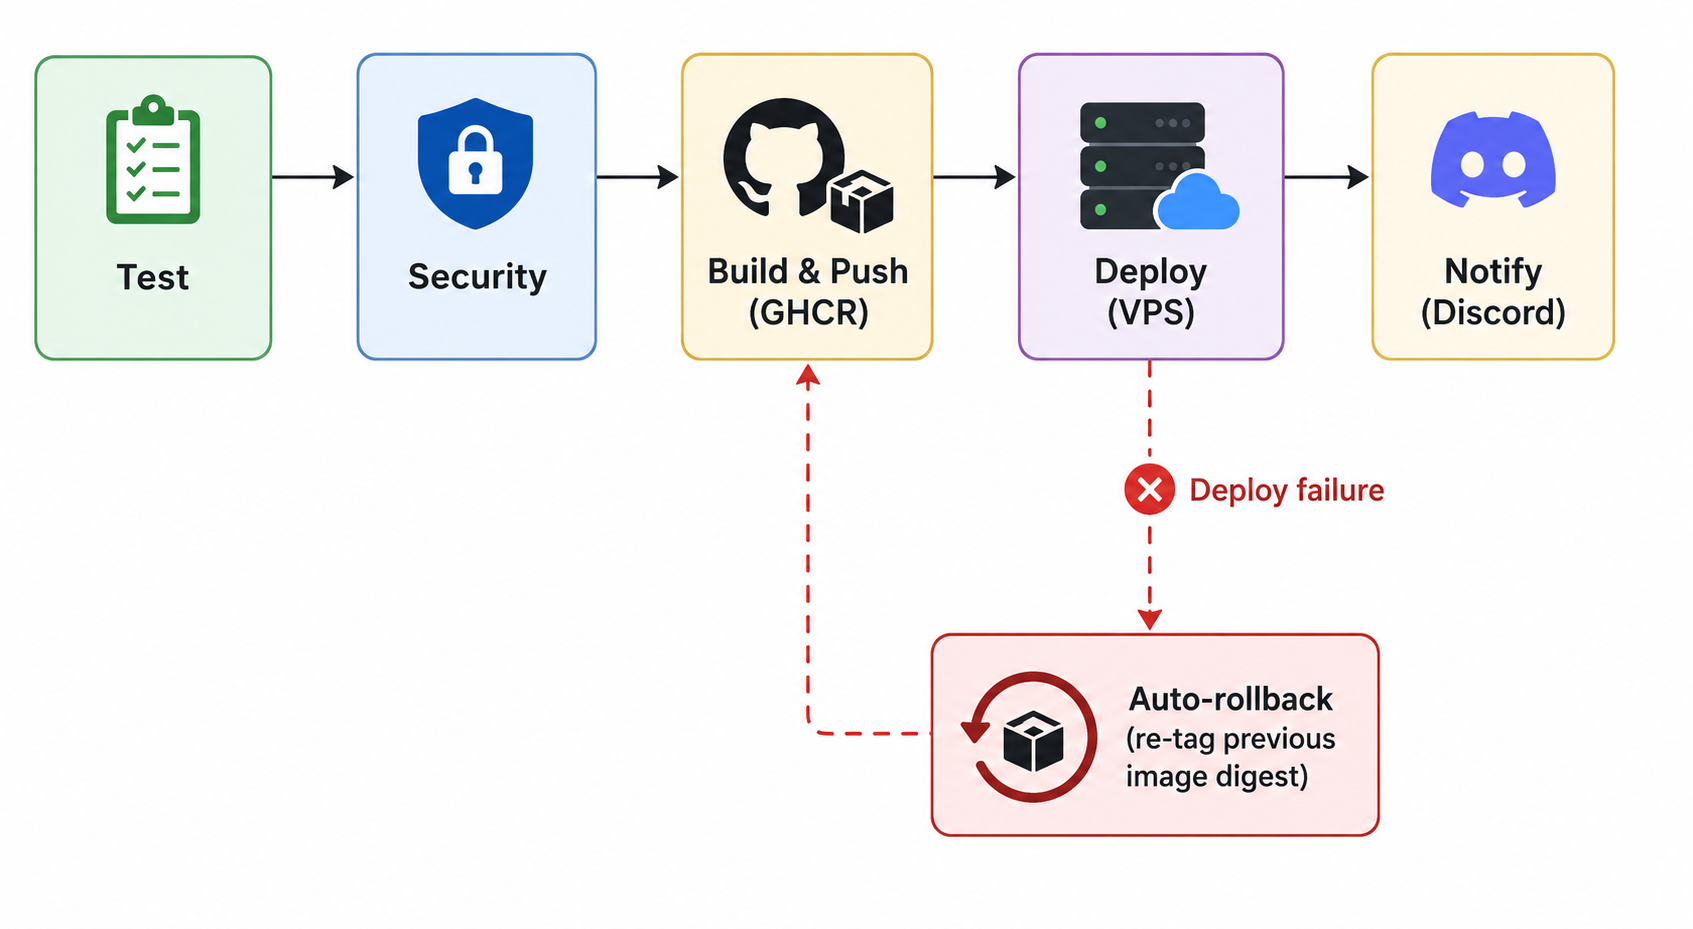
\includegraphics[width=0.9\textwidth]{img/PipelineDiagram.png}
    \caption{GitHub Actions CI/CD pipeline — five stages}
    \label{fig:cicd}
\end{figure}

\subsection{Stage Details}

\textbf{Stage 1 — Test:} Runs \texttt{npm ci}, \texttt{npm run lint}, and
\texttt{npm run test}. For frontend and admin, \texttt{--legacy-peer-deps} is used
due to React 19 peer dependency resolution.

\textbf{Stage 2 — Security:} Trivy filesystem scan and \texttt{npm audit}. Failure
blocks the build --- no deployment with known critical vulnerabilities.

\textbf{Stage 3 — Build and Push:} Docker Buildx builds the image and pushes it to
GitHub Container Registry (GHCR) with both \texttt{:latest} and a SHA-tagged version.
A second Trivy scan runs on the built image. For Next.js services, the API URL
environment variable is baked into the bundle at build time via Docker build argument.

\textbf{Stage 4 — Deploy:} The deploy stage connects to the VPS via SSH and executes
a rolling update:
\begin{enumerate}
    \item Snapshot the current image digest for rollback.
    \item Pull the new image and restart only the target service (\texttt{--no-deps}).
    \item Health check loop (18 retries $\times$ 5s = 90s timeout).
    \item On failure: re-tag the previous image digest as \texttt{:latest} and restart (automatic rollback).
    \item Cleanup dangling images.
\end{enumerate}

\textbf{Stage 5 — Notify:} Success or failure is reported to a Discord channel via
\texttt{sarisia/actions-status-discord}.

\subsection{GitHub Secrets}

\begin{longtable}{|m{4.5cm}|m{9cm}|}
    \hline
    \textbf{Secret}                   & \textbf{Purpose}               \\
    \hline
    \endhead
    \endfoot
    \endlastfoot
    \hline
    \texttt{VPS\_HOST}                & SSH target hostname            \\
    \hline
    \texttt{VPS\_USER}                & SSH user                       \\
    \hline
    \texttt{VPS\_SSH\_KEY}            & SSH private key                \\
    \hline
    \texttt{GHCR\_USER}               & GitHub Container Registry user \\
    \hline
    \texttt{GHCR\_PAT}                & GitHub Container Registry PAT  \\
    \hline
    \texttt{DISCORD\_WEBHOOK}         & Deployment notifications       \\
    \hline
    \texttt{NEXT\_PUBLIC\_{}API\_URL} & Baked into Next.js builds      \\
    \hline
    \caption{GitHub Actions secrets}
    \label{tab:secrets}
\end{longtable}

\section{Production Infrastructure}

\subsection{VPS Configuration}

The platform runs on a single OVH VPS (Ubuntu LTS) with Docker Compose managing
all services. The deployment path \texttt{/var/www/malltech/} contains the
\texttt{docker-compose.yml}, \texttt{Caddyfile}, \texttt{.env}, and the auto-healing
script.

\subsection{Network Topology}

All application containers share a Docker bridge network named \texttt{malltech}.
Only Caddy exposes ports 80 and 443 to the host. All other services use
\texttt{expose} (internal Docker network only). \texttt{mongo-express} is bound to
\texttt{127.0.0.1:8081} and is accessible only via SSH tunnel.

\subsection{TLS and HTTPS}

Caddy handles TLS automatically: on first start, it provisions Let's Encrypt
certificates for all configured domains, auto-renews before expiry, and redirects
HTTP requests to HTTPS.

\subsection{Data Persistence}

\begin{longtable}{|m{3cm}|m{3cm}|m{7.5cm}|}
    \hline
    \textbf{Volume}        & \textbf{Container} & \textbf{Purpose}              \\
    \hline
    \endhead
    \endfoot
    \endlastfoot
    \hline
    \texttt{mongodb\_data} & mongodb            & Database files                \\
    \hline
    \texttt{api\_storage}  & api                & Uploaded product images, PDFs \\
    \hline
    \texttt{caddy\_data}   & caddy              & TLS certificates              \\
    \hline
    \texttt{caddy\_config} & caddy              & Caddy runtime configuration   \\
    \hline
    \texttt{netdata\_*}    & netdata            & Monitoring data               \\
    \hline
    \caption{Docker volume mapping}
    \label{tab:volumes}
\end{longtable}

\section{Monitoring and Auto-Healing}

\subsection{Netdata}

Netdata runs as a container with access to \texttt{/proc} and \texttt{/sys} for
system-level metrics (CPU, RAM, disk, network) and to the Docker socket for
container-level metrics. The Netdata dashboard is accessible at
\texttt{monitor.domain.com} behind Caddy basic auth. Alerts are pre-configured
for high CPU/memory usage, disk space thresholds, and container health transitions.

\subsection{Auto-Healing Script}

The healing script (\texttt{malltech-heal.sh}) is mounted into the Netdata container
as a custom alarm action. When Netdata fires a \texttt{critical} alert on a container,
the script:

\begin{enumerate}
    \item Checks a 5-minute cooldown between restart attempts.
    \item Checks whether the maximum restart attempt count (2) has been reached.
    \item Restarts the container via Docker Compose.
    \item Logs the restart and notifies via Discord.
\end{enumerate}

This provides a self-healing first response layer before manual intervention is required.


\section*{Conclusion}
This chapter covered the full quality and delivery pipeline: unit and E2E testing
with Jest/Supertest, automated security scanning with Trivy and npm audit, a
five-stage GitHub Actions CI/CD pipeline with zero-downtime rolling deployment and
automatic rollback, the Docker-based production infrastructure on OVH, and the
Netdata + auto-healing monitoring layer. Together these practices ensure reliable,
repeatable, and secure delivery of the platform.
